\section{Spectral Function at High (Relative) Momenta\label{sec:specfunc}}
\subsection{Singlet and Triplet Spectral Functions}
It is the aim of the calculation of the spectral function to obtain 
information about the influence of the short-range repulsive interaction on 
the relative wave functions at short distance and therefore on the  
high-momentum parts of the spectral function to which they give rise. 
This influence will be largest when the two protons come close, 
\ie\ in relative $l=0$ and to a less extent, $l=1$. This is indeed clearly 
shown by the size of the defect functions in fig.~\ref{fig:defectAll}. 
Therefore, given the spectra and the corresponding shell model two-proton 
removal amplitudes, as discussed in the previous section and shown in 
table~\ref{tab:CveertienAmp}, it is meaningful to ask to what extent these 
correspond to the removal of a singlet-S or triplet-P pair.


The largest defect function is that of the $^1S_0$ partial wave 
(see fig.~\ref{fig:defectAll}), so
the most pronounced effect of SRC will be visible in this partial wave.
A quantity that will be of interest is therefore the `$^1S_0$-removal
spectral function' defined as
%
	\begin{equation}
		S_{^1S_0}(\omega)
	=
		\sum_m
		|\ME< {}^{14}{\rm C}^m | (aa)_{^1S_0} | {}^{16}{\rm O} >| ^2
	\;
		\delta( \omega - E^m )
	\label{eq:S1S0}
	\;,
	\end{equation}
%
in which the operator $(aa)_{^1S_0}$ annihilates two particles coupled to
 $^1S_0$. This removed pair will still be characterized by the radial 
quantum numbers $n$ of the relative motion and the quantum numbers $N$ and 
 $L$ of its center-of-mass motion.
The spectral function (\ref{eq:S1S0}) can be expressed in terms of the 
recoupling coefficients of (\ref{eq:Cab}) and the two-nucleon removal 
amplitudes $X$ of (\ref{eq:g2}) by a simple recoupling\cite{Ed57}
%
	\begin{equation}
		S_{^1S_0}(\omega)
	=
		\sum_{m,J}
		\sum_{ab,cd}
		X_{ab}^m
		\sum_{ij}
		\tilde{C}^{ab;J}_{Si}
		\tilde{C}^{cd;J}_{Sj}
		X_{cd}^m
		\delta( E - E_J^m )
		\;,
	\label{eq:S1S01}
	\end{equation}
%
where the coupling coefficients $\tilde{C}$ had been defined (for general
partial waves) as
%
	\begin{equation}
		\tilde{C}^{ab;J}_{SnlNL\lambda}
	=
		\sum_{J'}
		(-)^{ L -\lambda +J' + S}
		\zesJ( L, l, \lambda, S, J, J' )
		C^{ab;J}_{nNL(lS)J'}
	\label{eq:Ctilde}
	\;.
	\end{equation}
%
In (\ref{eq:S1S01}) the spin $S$ is set to zero.
The easiest way to calculate the $^1S_0$-hole spectral function (\ref{eq:S1S0})
is to rewrite the expression (\ref{eq:S1S0}) into the form
%	
	\begin{equation}
		S_{^1S_0}(\omega)
	=
		\frac{1}{\pi}
		{\rm Im}
	\;
		\sum_J
		(2J+1)
	\;
		v_{ab;J}
		G^{II}_{ab;cdJ}(\omega) 
		v_{cd;J}
	\label{eq:S1S0R}
	\;,
	\end{equation}
%
where the vector $v_{ab;J}$ is obtained by inverting (\ref{eq:Ctilde})
with fixed values of $n$, $N$, $L$ and of course $(lS)J'$. In the calculations
presented here $n$, $N$ and $L$ are chosen to have the lowest possible values.
The advantage of rewriting (\ref{eq:S1S01}) in the form (\ref{eq:S1S0R}) lies
in its similarity to the expression for the particle-hole response functions
(\ref{eq:defS}). Now a continuous DRPA calculation can be performed directly 
avoiding the procedure of calculating the amplitudes $X$ with the contour 
integration method of (\ref{eq:contour}).

%%%%%%%%%%%%%%
\begin{figure}
\centerline{%
\epsfig{file=figures/lrstruct_1S0.ps, width=9cm}
}
\caption[]{%
The spectral function for removal of a $^1S_0$ pair (\ref{eq:S1S0}). The residual
quantum numbers of the pair are $n=0$, $N=0$ and $L=J$. Only the the first peaks
are discernible. The finite width is obtained by setting $\eta$ equal to $0.5$ 
MeV in the `continuous' DRPA calculation. The peak labeled with `$2^+/0^+$' 
contains a small shoulder of $0^+$ strength.
\label{fig:S1S0}}
\end{figure}
%%%%%%%%%%%%%%
%%%%%%%%%%%%%%
\begin{figure}
\centerline{%
\epsfig{file=figures/lrstruct_3P.ps, width=9cm}
}
\caption[]{%
The spectral function for removal of a $^3P_0$ pair, \cf\ (\ref{eq:S1S0}) and 
fig.~\ref{fig:S1S0}. The residual
quantum numbers of the pair are $n=0$, $N=0$ and $L=0$ for the solid line and 
 $L=1$ for the dashed line. The $L=0$ contribution consists solely of negative
parity states, while the $L=1$ contribution consists exclusively of positive
parity states.
\label{fig:S3P}}
\end{figure}
%%%%%%%%%%%%%%
The `$^1S_0$ removal spectral function' (\ref{eq:S1S0}) is plotted
in fig.~\ref{fig:S1S0}. The contributions of the first two states in the 
the two-hole spectrum of table~\ref{tab:CveertienAmp} are visible as peaks.
The second peak mainly originates from the second $2^+$ state. 
Experimentally\cite{Ajz1617,Ajz1315} the $2^+_2$ state is at $8.32$~MeV and the 
$0^+_2$ state at $9.75$~MeV, so they could be separated with sufficiently good 
energy resolution. The $1^-$ contribution is spread over a wide energy region.
Analogous to expression
(\ref{eq:S1S0}), a `$^3P$ removal spectral function' could be 
defined (putting $l=1$ and $S=1$). This function is plotted in
fig.~\ref{fig:S3P}. In this case the contributions with different 
center-of-mass angular momenta $L$ manifest themselves mainly at different 
energies.

\subsection{Spectral Function for the Lowest $0^+$ and $2^+$ States}
{\def\pone{\rvec{p}'_1}\def\ptwo{\rvec{p}'_2}\def\q{\rvec{q}}%
The spectral function (\ref{eq:SpecFuncW}) is in principle a function of 
seven variables (two 3-vectors and one energy). So, it can not be 
plotted directly. 
Constraints have to be imposed to find the interesting characteristics.
Like in the analysis of \eepp\ data on $^{12}$C at 
NIKHEF-K\cite{Kes93,GP91}, the virtual photon is supposed to couple to
one of the protons. 
The momenta in (\ref{eq:SpecFuncW}) are the momenta within the nucleus, and
the detection gives no clear correspondence between these and the observed 
momenta $\pone$ and $\ptwo$. Therefore, in the approximation of the virtual
photon coupling only to one of the protons the cross-section will depend 
on the coherent sum of two amplitudes. Expressed in terms of spectral 
functions the relevant quantity is
%
	\begin{eqnarray}
	\lefteqn{%
		\hat{S}(\pone, \ptwo, E)
	=} 
	\label{eq:Shat}
	&&\\
	&&
		 S( \pone-\q, \ptwo, \pone-\q, \ptwo, E )
		+S( \pone-\q, \ptwo, \pone, \ptwo-\q, E )
	\nonumber \\
	&+&
		 S( \pone, \ptwo-\q, \pone-\q, \ptwo, E )
		+S( \pone, \ptwo-\q, \pone, \ptwo-\q, E ) 
	\nonumber
	\;,
	\end{eqnarray}
where the vector $\q$ is the momentum of the virtual photon. 
} 

%\subsection{Example}
As an example, the spectral function is plotted at the energies
of the $0^+$ ground state and the first $2^+$ excited state.
This means that in fact the strength that multiplies the delta function in
(\ref{eq:SpecFunc}) at the first $0^+$ and $2^+$ state energies is plotted. 
These states
are also visible in the figures \ref{fig:S1S0} and~\ref{fig:S3P}, but there
they have finite width. The contour integration method  (\ref{eq:contour})
provides directly the amplitudes of these states.
The strength that multiplies the delta function still depends on the 
momenta, \cf\ 
(\ref{eq:Shat}). A way to plot $\hat{S}$ is to
fix the angles of the momenta at some reasonable configuration of detectors,
\eg\ corresponding  to the measurements at NIKHEF\cite{Prop}. 
%In this way
%we see in essence what the effect of the correlations is in the spectral 
%function. 

This procedure is followed in fig.~\ref{fig:sfC1}, where the 
difference of the short-range effects of the RSC and Bonn-A potentials 
are visualized.
In the plots labeled `No SRC' just harmonic oscillators have been taken for 
the relative wave functions in the spectral function. One clearly sees that 
these give no contribution at higher momenta.
%%%%%%%%%%%%%%
\begin{figure}
\centerline{%
\epsfig{file=figures/2psf/0+_none.ps, width=6cm}
\epsfig{file=figures/2psf/2+_none.ps, width=6cm}
}
\centerline{%
\epsfig{file=figures/2psf/0+_Reid.ps, width=6cm}
\epsfig{file=figures/2psf/2+_Reid.ps, width=6cm}
}
\centerline{%
\epsfig{file=figures/2psf/0+_OBEPA.ps, width=6cm}
\epsfig{file=figures/2psf/2+_OBEPA.ps, width=6cm}
}
\caption[]{%
Spectral function for fixed angles of the momenta. 
The vector $\rvec{q}$ is fixed at the $z$-axis, with length $313$ MeV/c.
The vectors $\rvec{p}_1$ and $\rvec{p}_2$ are in-plane with each other
and with $\rvec{q}$ at respectively $-49$ and $123$ degrees.
The plotted function is 
$\hat{S}(\rvec{p}_1, \rvec{p}_2, E)|\rvec{p}_1|^2|\rvec{p}_2|^2$ 
(\ref{eq:Shat}),
where $E$ is fixed to the the first $0^+$ and the first $2^+$, respectively.
In the first two plots no SRC effects were taken into account. The second
line contains plots, where the SRC are taken into account by means of the
Reid defect functions (\cf\ fig.~\ref{fig:defectAll}) while the third line 
displays the effect of the Bonn-A defect functions.
\label{fig:sfC1}}
\end{figure}
%%%%%%%%%%%%%%
The high-momentum part of the spectral function is about a factor two larger 
for the Bonn potential than for the Reid in the momentum range around 
$3$--$5$~fm$^{-1}$. The short-range correlations give rise to a spectral 
function which is clearly distinct from that without SRC.
%%%%%%%%%%%%%%
\begin{figure}
\centerline{%
\epsfig{file=figures/2psf/sf_obepc.ps, width=6cm}
\epsfig{file=figures/2psf/sf_2+_obepc.ps, width=6cm}
}
\centerline{%
\epsfig{file=figures/2psf/sf_kk.ps, width=6cm}
\epsfig{file=figures/2psf/sf_2+_kk.ps, width=6cm}
}
\centerline{%
\epsfig{file=figures/2psf/sf_omy.ps, width=6cm}
\epsfig{file=figures/2psf/sf_2+_omy.ps, width=6cm}
}
\caption[]{%
Same figure as fig.~\ref{fig:sfC1} for different short-range correlation
parts. Note that the scale of plots where the KK and OMY correlation functions
of fig.~\ref{fig:KKOMY} are used, 
is different from the scale in the plots with defect functions.
\label{fig:sf2C1}}
\end{figure}
%%%%%%%%%%%%%%
In fig.~\ref{fig:sf2C1} the same result is shown with the
Bonn-C defect functions. No significant difference with the
Bonn-A calculation is found. 
The KK (\ref{eq:KK}) and OMY (\ref{eq:OMY}) correlation
functions yield for the transition to 
the ground state a much larger spectral function, 
already at low relative momenta. Also for the transition to the first $2^+$ 
the spectral function using OMY shows more SRC effects than the ones using 
more realistic potentials.
